\documentclass{beamer}
\usepackage{graphicx}

\definecolor{uoanavy}{RGB}{0,60,127}

\usetheme{Frankfurt}
\usecolortheme{orchid}
\setbeamertemplate{navigation symbols}{}
\setbeamercolor{structure}{fg=uoanavy}
\setbeamercolor{blocktitle}{fg=uoanavy}

\usepackage{pgfplots}

\usepackage{doi}

\title{Hamiltonian Monte Carlo on the\\Space of Phylogenies}
\author{Arman Bilge \\ \scriptsize \texttt{abil933@aucklanduni.ac.nz} \\ Centre for Computational Evolution \\ The University of Auckland}

\institute{\small Joint work with Vu Dinh and Erick Matsen \\ \scriptsize Fred Hutchinson Cancer Research Center}
\date{June 20, 2016}

\usepackage{mathtools}
\newcommand{\dd}{\, \mathsf{d}}
\renewcommand{\vec}[1]{\ensuremath{\boldsymbol{\mathbf{#1}}}}
\newcommand{\mat}[1]{\ensuremath{\boldsymbol{\mathbf{#1}}}}
\newcommand{\op}[1]{\ensuremath{\boldsymbol{\mathbf{#1}}}}
\newcommand{\norm}[1]{\ensuremath{\mathcal{N}\left(#1\right)}}

\usepackage{algorithm}
\usepackage{algpseudocode}

\setbeamertemplate{itemize items}[default]
\setbeamertemplate{enumerate items}[default]

\begin{document}

\frame{\titlepage}

\section{Introduction}

\stepcounter{subsection}
\begin{frame}{Motivation}
	\begin{itemize}
		\item Bayesian statistics has \textbf{transformed evolutionary biology}
		\begin{itemize}
			\item Divergence dating and clock rate estimation
			\item Inference of demographics and population history
			\item Phylodynamic and epidemiological parameters
		\end{itemize}
		\pause
		\item Want to \textbf{sample phylogenetic trees} according to their probability given the data, $P\left(\mathcal{T} \mid D\right)$ \pause
		\item Need a way to \textbf{efficiently explore} different trees
	\end{itemize}
\end{frame}

\stepcounter{subsection}
\begin{frame}{Current State-of-the-Art}
	\begin{itemize}
		\item Metropolis--Hastings Markov chain Monte Carlo (\textbf{MCMC})
		\item Imagine a robot taking a \textbf{random walk} \pause
		\item That's just unbearably slow
		\item Analyses capped at about 1000 taxa\pause
		\item \textbf{But suppose we gave our robot a pair of skis...}
	\end{itemize}
\end{frame}

\stepcounter{subsection}
\begin{frame}{Cooker, an Aspiring Skier}
  \centering
	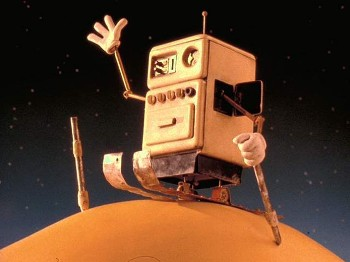
\includegraphics[width=0.75\textwidth]{skier}
\end{frame}

\section{Hamiltonian Monte Carlo}

\stepcounter{subsection}
\begin{frame}{Physics Primer}
	\begin{columns}
		\begin{column}{.5\textwidth}
			\begin{definition}
				Let \small
				\begin{itemize}
					\item $\vec{q}$ be the robot's position
					\item $\vec{v}$ be its velocity
					\item $\mat{M}$ be its mass
					\item $U\left(\vec{q}\right)$ be its potential energy
					\item $K\left(\vec{p}\right)$ be its kinetic energy
				\end{itemize}

				\normalsize Then the Hamiltonian $\mathcal{H}$ is
				\begin{equation*}
					\mathcal{H}\left(\vec{q},\vec{p}\right) = U\left(\vec{q}\right) + K\left(\vec{p}\right)
				\end{equation*}
			\end{definition}
      \visible<2>{
        \begin{itemize}
          \item Describes robot's motion
          \item $\mathcal H$ (energy) is conserved
        \end{itemize}
      }
		\end{column}
		\begin{column}{.5\textwidth}
      \centering
			\begin{tikzpicture}
				\node at (0, 0) {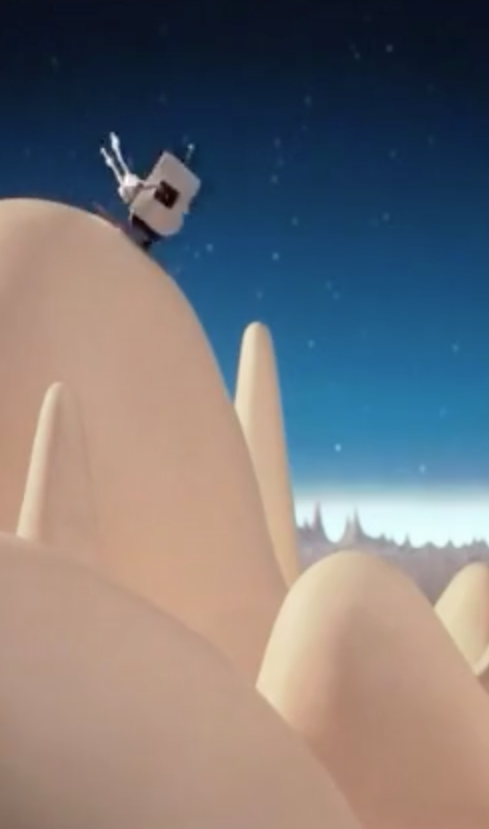
\includegraphics[width=0.75\textwidth]{primer}};
        \draw[thick,<-] (-1,1.2) -- (-1, -3);
        \node at (-0.5, -1) {$U\left(\vec{q}\right)$};
        \draw[thick,->] (-2,-3.2) -- (2, -3.2);

				\node at (0, -2.9) {$\vec{q}$};
        \draw[thick,->,white] (-0.5,1.5) -- (0, 1);
        \node[white] at (0.8, 1.35) {$\vec{p}=\mat{M}\vec{v}$};

				\node[white] at (0, 3) {$K\left(\vec{p}\right) = \frac{1}{2}\vec{p}^T \mat{M}^{-1} \vec{p}$};
			\end{tikzpicture}
		\end{column}
	\end{columns}
  \pause
\end{frame}

\stepcounter{subsection}
\begin{frame}[t]{The Operations}
  \textbf{Push in a random direction}
\end{frame}

\stepcounter{subsection}
\begin{frame}[t]{The Operations}
  \textbf{Ski!}
\end{frame}

\stepcounter{subsection}
\begin{frame}[t]{The Operations}
  \textbf{Flip direction}
\end{frame}

\stepcounter{subsection}
\begin{frame}{Hamiltonian Monte Carlo}

  \textbf{How do we make a stats problem into a physics problem?}
  \pause
  \begin{itemize}
    \item Every location $\vec q$ maps to some model parameters \pause
    \item Elevation at $\vec q$ is $-\log{P\left(\mathcal{T}, \vec\theta \mid D\right)}$
    \item Locations with \textbf{high elevation} have \textbf{low probability}
    \item Locations with \textbf{low elevation} have \textbf{high probability} \pause
    \item Run the HMC algorithm
  \end{itemize}

\end{frame}

\stepcounter{subsection}
\begin{frame}{HMC Algorithm}

  \begin{enumerate}
    \item Choose random momentum $\vec{p}$ for robot
    \item Simulate its motion using \textbf{leapfrog integrator}
    \item Flip its momentum \pause
    \item Let $a = \min\left(1, \exp\left(\mathcal{H}\left(\vec{q}, \vec{p}\right) - \mathcal{H}\left(\vec{q}^\prime, \vec{p}^\prime\right)\right)\right)$
        \begin{itemize}
            \item Remember that $\mathcal{H}$ is approximately conserved!
        \end{itemize}
    \item With probability $a$ accept its position; \\ otherwise reject and put it back where it was \pause
    \item Flip its momentum again
    \item Save its position as sample from target distribution \pause
    \item Repeat forever
  \end{enumerate}

\end{frame}

\stepcounter{subsection}
\begin{frame}{Scalability}

  \textbf{Running a physics simulator seems like a lot of work! \\ Why should we bother?}

  \pause

  \begin{theorem}[Creutz 1988]
    Consider a model with $n$ variables. \\
    Then (under simplifying assumptions) the computation time is
    \begin{itemize}
      \item $\mathcal{O}\left(n^2\right)$ for MCMC; and
      \item $\mathcal{O}\left(n^\frac{5}{4}\right)$ for HMC.
    \end{itemize}
  \end{theorem}

  \pause

  In practice this means \textbf{doubling the number of variables} increases computation time by
  \begin{itemize}
    \item \textbf{4x} for MCMC
    \item \textbf{$<$2.5x} for HMC!
  \end{itemize}

\end{frame}

\section{phyloHMC}

\stepcounter{subsection}
\begin{frame}{Beyond Euclidian Spaces}

That is all very well for ordinary Euclidian spaces, but the \\ \textbf{space of phylogenies} is much more complicated.
\begin{itemize}
  \item All possible topologies with all possible branch lengths
\end{itemize}
\vspace{16pt}
\pause

For a fixed topology, the branch lengths form a Euclidian space.
\vspace{16pt}
\pause

\textbf{How can we move continously between topologies?}

\end{frame}

\stepcounter{subsection}
\begin{frame}{Moving Between Phylogenies}
  \centering
  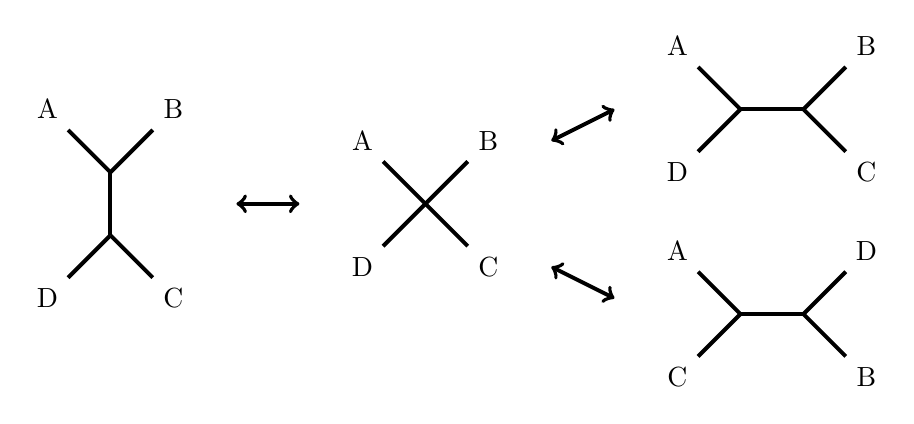
\begin{tikzpicture}[scale=0.8, line width=0.5mm]
    \node [] (0) at (-1, 1) {A};
    \node [] (1) at (1, -1) {C};
    \node [] (2) at (1, 1) {B};
    \node [] (3) at (-1, -1) {D};
    \node [] (4) at (-2, 0) {};
    \node [] (5) at (-3, 0) {};
    \node [] (6) at (-4, -1.5) {C};
    \node [] (7) at (-6, -1.5) {D};
    \node [] (8) at (-5, -0.5) {};
    \node [] (9) at (-5, 0.5) {};
    \node [] (10) at (-6, 1.5) {A};
    \node [] (11) at (-4, 1.5) {B};
    \node [] (12) at (2, 1) {};
    \node [] (13) at (3, 1.5) {};
    \node [] (14) at (2, -1) {};
    \node [] (15) at (3, -1.5) {};
    \node [] (16) at (4, -0.75) {A};
    \node [] (17) at (4, -2.75) {C};
    \node [] (18) at (5, -1.75) {};
    \node [] (19) at (6, -1.75) {};
    \node [] (20) at (7, -2.75) {B};
    \node [] (21) at (7, -0.75) {D};
    \node [] (22) at (4, 0.5) {D};
    \node [] (23) at (4, 2.5) {A};
    \node [] (24) at (5, 1.5) {};
    \node [] (25) at (6, 1.5) {};
    \node [] (26) at (7, 0.5) {C};
    \node [] (27) at (7, 2.5) {B};
    \draw (0) to (1);
    \draw (2) to (3);
    \draw [<->] (4.center) to (5.center);
    \draw (10) to (9.center);
    \draw (9.center) to (8.center);
    \draw (8.center) to (7);
    \draw (8.center) to (6);
    \draw (9.center) to (11);
    \draw [<->] (14.center) to (15.center);
    \draw [<->] (12.center) to (13.center);
    \draw (22) to (24.center);
    \draw (24.center) to (25.center);
    \draw (25.center) to (26);
    \draw (25.center) to (27);
    \draw (24.center) to (23);
    \draw (16) to (18.center);
    \draw (18.center) to (17);
    \draw (18.center) to (19.center);
    \draw (19.center) to (20);
    \draw (19.center) to (21);
  \end{tikzpicture}
  ``BHV space'' / ``NNI space''
\end{frame}

\begin{frame}{Leap-Prog Integrator}

  \begin{itemize}
    \item \textbf{Probabilistic generalization} of the leap-frog integrator
    \item When internal branch length goes to 0, \textbf{chooses randomly} from three adjacent phylogenies
  \end{itemize}

  \pause

  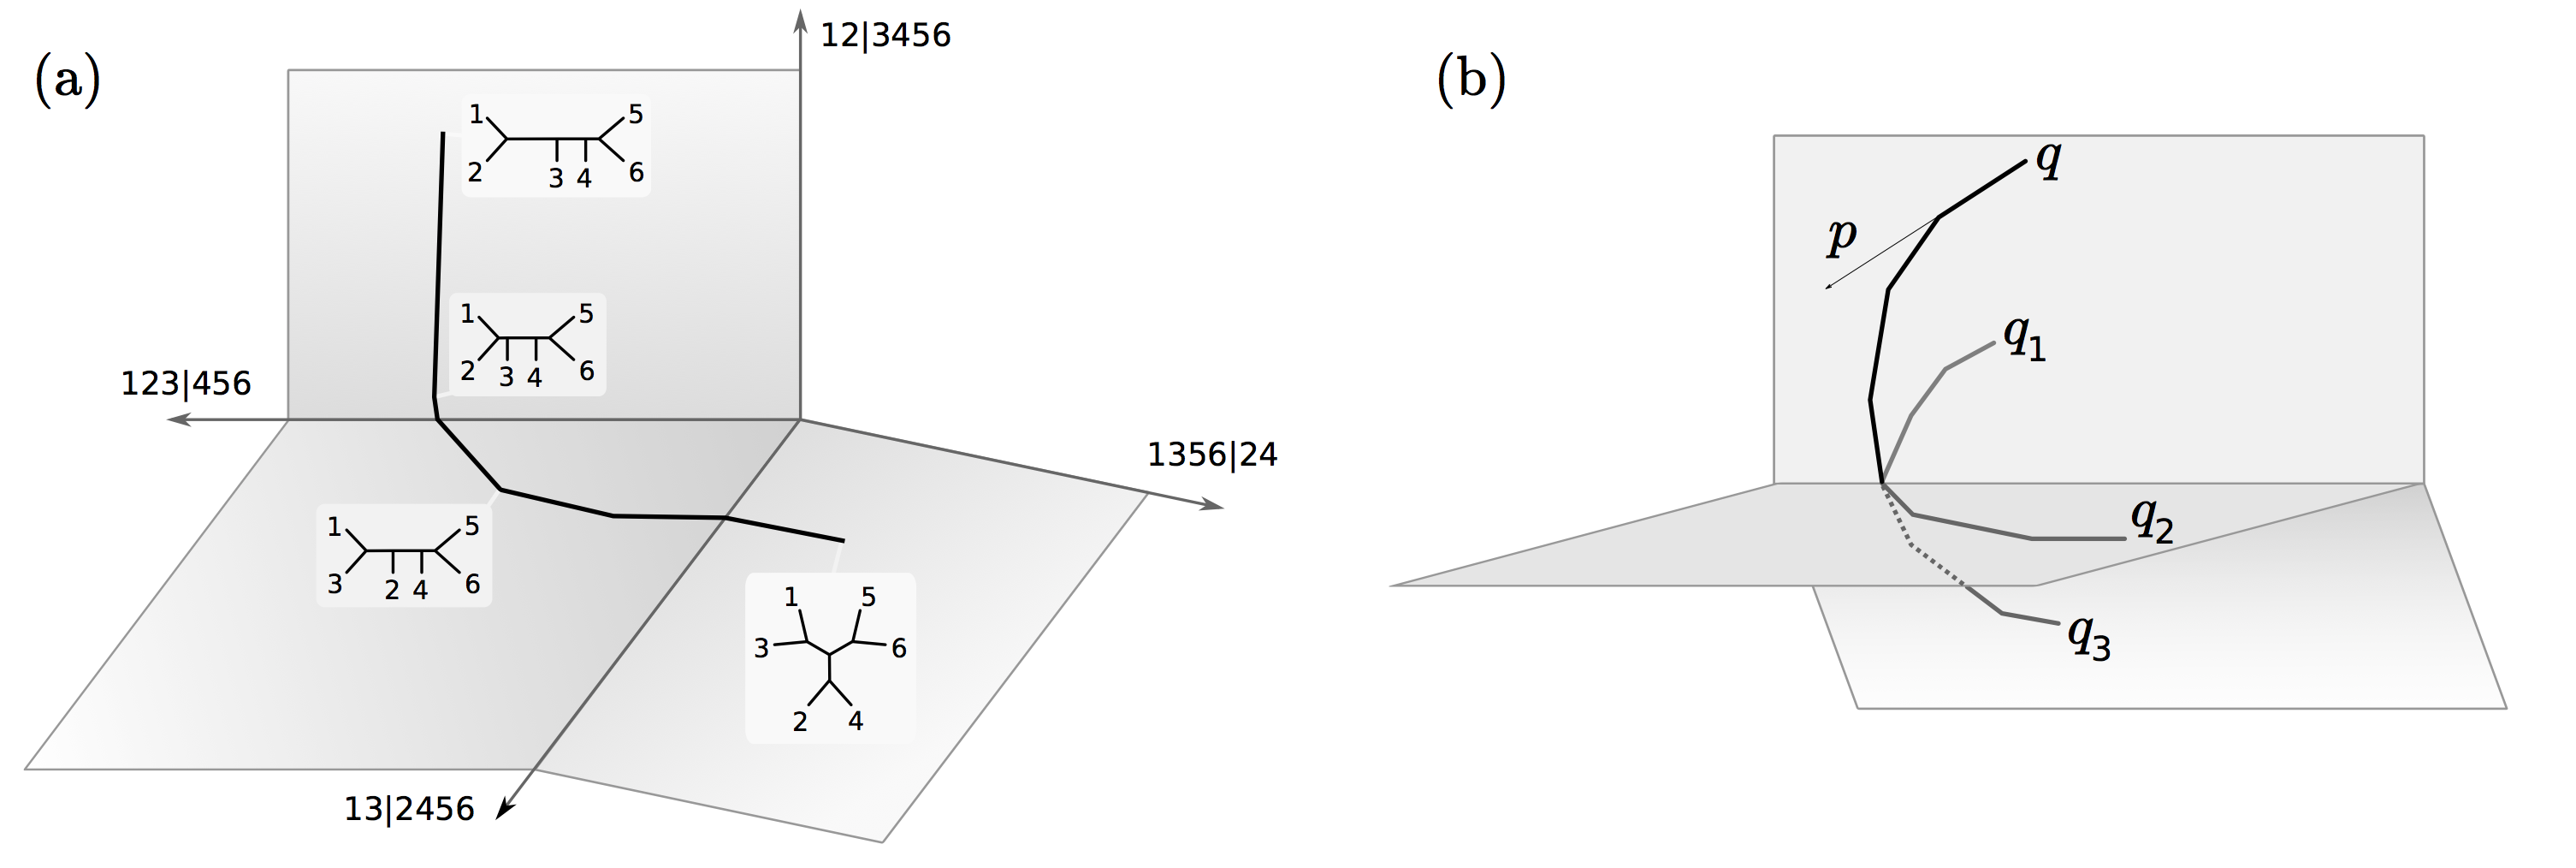
\includegraphics[width=\textwidth]{leap-prog.png}

\end{frame}

\stepcounter{subsection}
\begin{frame}{The Phylogenetic Ski Slope}

\end{frame}

\stepcounter{subsection}
\begin{frame}[fragile]{Acceptance Probability through Time}
  \begin{center}
    \input{acceptance.tex}
  \end{center}
\end{frame}

\stepcounter{subsection}
\begin{frame}[fragile]{Non-Differentiability in Target Distribution}
  \begin{center}
    \includegraphics[width=\textwidth]{nondiff.pdf}
  \end{center}
\end{frame}

\section{Conclusion}

\stepcounter{subsection}
\begin{frame}{Final Remarks}
  \begin{block}{Contributions}
    \begin{itemize}
      \item Generalized HMC to phylogenetic tree space
      \item Many ideas for leap-prog integrator with good performance
      \item Open source implementation at \texttt{www.github.com/armanbilge/phyloHMC}
    \end{itemize}
  \end{block}
  \pause
  \begin{block}{Current/Future Work}
    \begin{itemize}
      \item Prove practical leap-prog integrator is correct
      \item phyloHMC for rooted trees
      \item Efficient approximations to derivatives
      \item More sophisticated flavors of HMC
    \end{itemize}
  \end{block}
\end{frame}

\stepcounter{subsection}
\begin{frame}
  \begin{block}{These slides}
    \large \texttt{\doi{10.5281/zenodo.55957}}
  \end{block}
  \begin{block}{Thanks to}
    \begin{itemize}
      \item Alex Gavryushkin
      \item Allan Wilson Centre
      \item Evolution Conference
    \end{itemize}
  \end{block}
  \begin{block}{References}
    \footnotesize
    LJ Billera et al. \textit{Adv Appl Math} 27.4 (2001). \texttt{\doi{10.1006/aama.2001.0759}} \\
    M Creutz. \textit{Physical Review D} 38.4 (1988). \texttt{\doi{10.1103/PhysRevD.38.1228}} \\
    RM Neal. \textit{Handbook of Markov Chain Monte Carlo} Chapter 5 (2011).
  \end{block}
  \vspace{24pt}
  \centering\Large\textbf{Thank you!}
\end{frame}

\end{document}
